\documentclass[12pt]{article}
\usepackage[utf8]{inputenc}

\usepackage{enumitem}
\usepackage[margin=2cm]{geometry}

\usepackage{amsmath, amsfonts, amssymb}
\usepackage{graphicx}
\usepackage{tikz}
\usepackage{pgfplots}
\usepackage{multicol}

\usepackage{comment}
\usepackage{url}
\usepackage{calc}

\usepackage{titlesec}
\titleformat{\section}[frame]
{\normalfont\scshape}
{\thesection}{8pt}{\centering}

\usepackage{array}

\pgfplotsset{compat=1.16}

%\usepackage[margin=1cm]{cloze}

\usepackage[thmmarks]{ntheorem}

% MATH commands
\newcommand{\bC}{\mathbb{C}}
\newcommand{\bR}{\mathbb{R}}
\newcommand{\bN}{\mathbb{N}}
\newcommand{\bQ}{\mathbb{Q}}
\newcommand{\bZ}{\mathbb{Z}}
\newcommand{\bT}{\mathbb{T}}
\newcommand{\bD}{\mathbb{D}}

\newcommand{\cL}{\mathcal{L}}
\newcommand{\cM}{\mathcal{M}}
\newcommand{\cP}{\mathcal{P}}
\newcommand{\cH}{\mathcal{H}}
\newcommand{\cB}{\mathcal{B}}
\newcommand{\cK}{\mathcal{K}}
\newcommand{\cJ}{\mathcal{J}}
\newcommand{\cU}{\mathcal{U}}
\newcommand{\cO}{\mathcal{O}}
\newcommand{\cA}{\mathcal{A}}
\newcommand{\cC}{\mathcal{C}}

\newcommand{\fK}{\mathfrak{K}}
\newcommand{\fM}{\mathfrak{M}}

\newcommand{\ga}{\left\langle}
\newcommand{\da}{\right\rangle}
\newcommand{\oa}{\left\lbrace}
\newcommand{\fa}{\right\rbrace}
\newcommand{\oc}{\left[}
\newcommand{\fc}{\right]}
\newcommand{\op}{\left(}
\newcommand{\fp}{\right)}

\newcommand{\ra}{\rightarrow}
\newcommand{\Ra}{\Rightarrow}

\renewcommand{\Re}{\mathrm{Re}\,}
\renewcommand{\Im}{\mathrm{Im}\,}
\newcommand{\Arg}{\mathrm{Arg}\,}
\newcommand{\Arctan}{\mathrm{Arctan}\,}
\newcommand{\sech}{\mathrm{sech}\,}
\newcommand{\csch}{\mathrm{csch}\,}
\newcommand{\Log}{\mathrm{Log}\,}
\newcommand{\cis}{\mathrm{cis}\,}

\newcommand{\ran}{\mathrm{ran}\,}
\newcommand{\bi}{\mathbf{i}}
\newcommand{\Sp}{\mathrm{span}\,}
\newcommand{\Inv}{\mathrm{Inv}\,}
\newcommand\smallO{
  \mathchoice
    {{\scriptstyle\mathcal{O}}}% \displaystyle
    {{\scriptstyle\mathcal{O}}}% \textstyle
    {{\scriptscriptstyle\mathcal{O}}}% \scriptstyle
    {\scalebox{.7}{$\scriptscriptstyle\mathcal{O}$}}%\scriptscriptstyle
  }
\newcommand{\HOL}{\mathrm{Hol}}
\newcommand{\cl}{\mathrm{clos}}
\newcommand{\ve}{\varepsilon}

\tikzstyle{myboxT} = [draw=black, fill=black!0,line width = 1pt,
    rectangle, rounded corners = 0pt, inner sep=8pt, inner ysep=8pt]
    
\newcommand{\MyC}[1]{\begin{tikzpicture}
\node (boxIntro) at (0,0) {};
\node [myboxT](Intro) at (boxIntro){%
	\begin{minipage}{0.9\textwidth}
	#1
	\end{minipage}};
\end{tikzpicture}}

%%%%  Environnement exer et solutionnaire
{\theorembodyfont{}
\theoremstyle{plain}
\theoremseparator{\textbf{.}}
\theoremsymbol{}
\newtheorem{exer}{\textbf{Exercise}}}

{\theorembodyfont{\color{blue}}
\theoremstyle{plain}
\theoremseparator{\textbf{:}}
\theoremsymbol{$\square$}
\newtheorem*{sol}{\textbf{Solution}}}

{\theorembodyfont{\color{blue}}
\theoremstyle{plain}
\theoremseparator{\textbf{:}}
\theoremsymbol{$\qed$}
\newtheorem*{solWP}{\textbf{Solution}}}

{\theorembodyfont{\color{blue}}
\theoremstyle{plain}
\theoremseparator{\textbf{:}}
\theoremsymbol{$\qed$}
\newtheorem*{hint}{\textbf{Hints}}}

\renewcommand*{\theexer}{\arabic{exer}}
\renewcommand*{\thesol}{\arabic{sol}}
\renewcommand*{\thesolWP}{\arabic{solWP}}
\renewcommand*{\thehint}{\arabic{hint}}

%%% Ignorer les solutions
\excludecomment{sol}
\excludecomment{solWP}
\excludecomment{hint}

\newcommand{\headHW}[4]{%
	\noindent \hrulefill \\
	MATH-#1 #2 \\
	#3 #4
	
}

\makeatletter
\DeclareFontFamily{U}{tipa}{}
\DeclareFontShape{U}{tipa}{m}{n}{<->tipa10}{}
\newcommand{\arc@char}{{\usefont{U}{tipa}{m}{n}\symbol{62}}}%

\newcommand{\arc}[1]{\mathpalette\arc@arc{#1}}

\newcommand{\arc@arc}[2]{%
  \sbox0{$\m@th#1#2$}%
  \vbox{
    \hbox{\resizebox{\wd0}{\height}{\arc@char}}
    \nointerlineskip
    \box0
  }%
}
\makeatother

\newcount\QO
\newcounter{QT}
\newcounter{QTh}
\newcounter{QF}
\newcounter{QFi}
\newcounter{QS}
\newcounter{QSe}
\newcounter{QE}
\newcounter{QN}
\newcounter{QTe}

\begin{document}
	\noindent \hrulefill \\
	MATH-331 Introduction to Real Analysis \hfill Created by P.-O. Paris{\'e}\\
	Homework 04 \hfill Fall 2021\\\vspace*{-0.7cm}
	
	\noindent\hrulefill
	
	\noindent Due date: October 25${}^{\text{th}}$ 1:20pm \hfill Total: \hspace{0.3cm}/70.
	
\vspace*{0.5cm}

	\bgroup \renewcommand{\arraystretch}{1.5}
\begin{table}[h]
\centering
\begin{tabular}{|m{1.5cm}|>{\centering\arraybackslash}p{0.75cm}|>{\centering\arraybackslash}p{0.75cm}|>{\centering\arraybackslash}p{0.75cm}|>{\centering\arraybackslash}p{0.75cm}|>{\centering\arraybackslash}p{0.75cm}|>{\centering\arraybackslash}p{0.75cm}|>{\centering\arraybackslash}p{0.75cm}|>{\centering\arraybackslash}p{0.75cm}|>{\centering\arraybackslash}p{0.75cm}|>{\centering\arraybackslash}p{0.75cm}|}
\hline
Exercise & 1 (5) & 2 (5) & 3 (5) & 4 (5) & 5 (10) & 6 (10) & 7 (5) & 8 (5) & 9 (5) & 10 (10) \\
\hline
Score & & & & & & & & & &  \\\hline
\end{tabular}
\caption{Scores for each exercises}
\end{table}
\egroup
	
\vspace*{0.5cm}

{\bf Instructions:} You must answer all the questions below and send your solution by email (to \url{parisepo@hawaii.edu}). If you decide to not use {\LaTeX} to hand out your solutions, please be sure that after you scan your copy, it is clear and readable. Make sure that you attached a copy of the homework assignment to your homework. 

\noindent If you choose to use {\LaTeX}, you can use the template available on the course website.

\noindent No late homework will be accepted. No format other than PDF will be accepted. Name your file as indicated in the syllabus.

\section{Writing problems}
For each of the following problems, you will be asked to write a clear and detailed proof. You will have the chance to rewrite your solution in your semester project after receiving feedback from me.

%% ---------------------------------------------
\begin{exer}
(5 pts)
Prove that, if $0 < x < \pi/2$, then $0 \leq \sin x \leq x$ with a geometric argument. [Hint: View $\sin x$ as a point on the unit circle in the first quadrant.]
\end{exer}
\begin{sol}
Suppose that $0 < x < \pi/2$. Consider the following geometric construction: 

	\begin{center}
	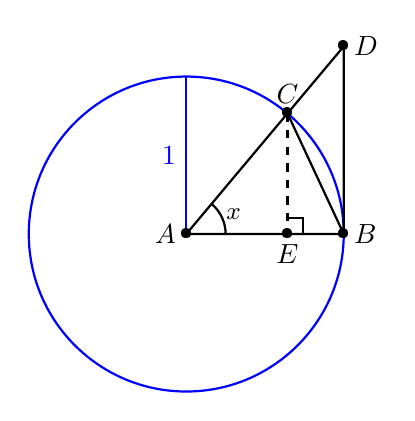
\begin{tikzpicture}
	\draw[blue, thick] (0,0) circle(2);
	\draw[blue, thick] (0,0) -- (0, 2)node[midway, left]{$1$};
	\draw[black, thick] ({2*cos(50)}, {2*sin(50)}) -- (2, {2*tan(50)})node{\textbullet} -- (2,0);
	\draw[black, thick] node{\textbullet} (0, 0) --  (2,0)node{\textbullet} -- ({2*cos(50)}, {2*sin(50)})node{\textbullet} -- (0,0);
	\draw[black, thick] (0,0)node[left]{$A$};
	\draw[black, thick] (2,0)node[right]{$B$};
	\draw[black, thick] ({2*cos(50)}, {2*sin(50)})node[above]{$C$};
	\draw[black, thick] (2, {2*tan(50)})node[right]{$D$};
	\draw[black, thick] (0.5, 0) arc(0:50:0.5);
	\draw[black, thick] (0.6, 0.25)node{\small $x$};
	\draw[black, dashed, thick] (({2*cos(50)}, {2*sin(50)}) -- (({2*cos(50)}, 0)node{\textbullet};
	\draw[black, thick] (({2*cos(50)}, 0)node[below]{$E$};
	\draw[black, thick] ({2*cos(50)+0.2}, 0) -- ({2*cos(50)+0.2}, 0.2) -- ({2*cos(50)}, 0.2);
	\end{tikzpicture}
	\end{center}
We see from this construction, that $\sin x = \overline{CE}$, that is $\sin x$ is the measure of the side $CE$. By Pythagorus Theorem, we have that $(\overline{CE})^2 + (\overline{EB})^2 = (\overline{CB})^2$. So, we obtain $(\overline{CE})^2 \leq \overline{CB})^2$ and since everything is positive, we get $\overline{CE} \leq \overline{CB}$. This means that $\sin x \leq \overline{CB}$. But, the line $\overline{CB}$ is the line that support that arc $\arc{CB}$ and so $\overline{CB} \leq \arc{CB}$. Since the circle has radius one, we have that $\arc{CB} = x$. Thus, we infer $\sin x \leq x$.
\end{sol}

%-----------------------------------------------
\begin{exer}
(5 pts)
Let $f : A \ra \bR$ and $g : B \ra A$ be two functions where $A, B \subset \bR$. Let $a$ be an accumulation point of $A$ and $b$ be an accumulation point of $B$. Suppose that
	\begin{itemize}
	\item $\lim_{t \ra b} g(t) = a$.
	\item there is a $\eta > 0$ such that for any $t \in B \cap (b - \eta ,  b + \eta )$, $g(t) \neq a$.
	\item $f$ has a limit at $a$.
	\end{itemize}
Prove that $f \circ g$ has a limit at $b$ and $\lim_{x \ra a} f(x) = \lim_{t \ra b} f(g(t))$. [This is the change of variable rule for limits.]
\end{exer}
\begin{sol}
Let $L$ be the limit at $a$ of $f$ and $M$ be the limit at $b$ of $g$.

We want to show that $f \circ g$ has a limit at $b$. Let $\varepsilon > 0$. Then there is a $\delta_1 > 0$ such that if $x \in A \cap (a - \delta_1 , a + \delta_1 ) \backslash \{ a \}$, then $|f(x) - L| < \varepsilon$. Also, there is a $\delta_2 > 0$ such that if $t \in B \cap (b - \delta_2 , b + \delta_2 )\backslash \{ b \}$, then $|g(t) - a| < \delta_1$. 

Put $\delta := \min \{ \delta_2 , \eta \}$. The second condition means $g(t)$ will never be equal to $a$ and so $|g(t) - a| > 0$ if $t$ is near $b$. Now, if $t \in B \cap (b - \delta , b + \delta )$, then $g(t) \in (a - \delta_1 , a + \delta_1 ) \backslash \{ a \}$. So, we get $|f(g(t)) - L| < \varepsilon$. In other words, $\lim_{t \ra b} f(g(t)) = L$.
\end{sol}

%-----------------------------------------------
\begin{exer}
(5 pts)
Let $f : [a, b] \ra \bR$ be continuous on $[a, b]$ and suppose that $f(x) = 0$ for each rational number $x$ in $[a, b]$. Prove that $f(x) = 0$ for all $x \in [a, b]$.
\end{exer}
\begin{sol}
Let $x \in [a, b]$. By the density of rational numbers in $[a, b]$, let $(x_n)$ be a sequence of rational numbers such that $x_n \ra x$. By the continuity of $f$, we must have that $f(x_n) \ra f(x)$ as $n \ra \infty$. But $f(x_n) = 0$ by assumption and so $f(x) = 0$.
\end{sol}

%-----------------------------------------------
\begin{exer}
(5 pts)
Let $f: [a, b] \ra \bR$ be continuous on $[a, b]$ and suppose that $f(c) > 0$ for some $c \in [a, b]$. Prove that there exist a number $\eta$ and an interval $[u, v] \subset [a, b]$ such that $f(x) \geq \eta$ for all $x \in [u, v]$.
\end{exer}
\begin{sol}
Suppose that $f$ is continuous on $[a, b]$ and that there exists a $c \in [a, b]$ such that $f(c) > 0$. Three cases:
	\begin{itemize}
	\item If $c = a$. In that case, with $\varepsilon = \frac{f(c)}{2}$, the continuity of the function at $a$ implies the existence of a $\delta > 0$ such that if $x \in [a, a + \delta )$, then $|f(x) - f(c)| < f(c)/2$. By the inverse triangle inequality, we get that if $x \in [a, a + \delta )$, then $f(x) \geq f(c) /2$. Now, put $u := a$, $v := a + \delta/2$, and $\eta := f(a)/2$.
	\item If $c = b$. Repeat the previous argument with $a$ replaced by $b$.
	\item If $c \in (a, b)$. In that case, with $\varepsilon = \frac{f(c)}{2}$, the continuity of the function at $a$ implies the existence of a $\delta > 0$ such that if $x \in (c - \delta , c + \delta ) \subset [a, b]$, then $|f(x) - f(c)| < \frac{f(c)}{2}$. By the inverse triangle inequality, we get $f(x) > f(c)/2$ when $x \in (c - \delta , c + \delta )$. Now, put $u := x - \delta/2$, $v = x + \delta/2$, and $\delta := f(c)/2$.
	\end{itemize}
\end{sol}

%-----------------------------------------------
\begin{exer}
(10 pts)
Let $f : \bR \ra \bR$ be a function that satisfies $f(x + y) = f(x) + f(y)$ for any real number $x$ and $y$.
	\begin{enumerate}[label=\textbf{\alph*)}]
	\item Suppose that $f$ is continuous at some point $c$. Prove that $f$ is continuous on $\bR$.
	\item Suppose that $f$ is continuous on $\bR$ and that $f(1) = k$. Prove that $f(x) = kx$ for all $x \in \bR$. [Hint: start with $x$ integer, then $x$ rational, and finally use Exercise 3.]
	\end{enumerate}
\end{exer}
\begin{sol}
\begin{enumerate}[label=\textbf{\alph*)}]
\item Suppose that $f$ is continuous at some point $c$. Remark that $f(0) = f(0 + 0) = 2 f(0)$ and so $f(0) = 0$. Also, from the characterization of continuous function in terms of limit, we have that $\lim_{h \ra 0} f(c + h) = f(c)$. Since $\lim_{h \ra 0} f(c) = f(c)$, this is equivalent to
	\begin{align*}
	\lim_{h \ra 0} f(c + h) - f(c) = \lim_{h \ra 0} f(c)
	\end{align*}
and so $\lim_{h \ra 0} f(h)$ exists and $\lim_{h \ra 0} f(h) = 0$. In other words, the function $f$ is continuous at $0$. Now, for any $h \in \bR$ and any $x_0 \in \bR$, we have
	\begin{align*}
	f(x_0 + h) - f(x_0) = f(x_0) + f(h) - f(x_0) = f(h)
	\end{align*}
and so the $\lim_{h \ra 0} f(x_0 + h) - f(x_0)$ exists and, moreover, we have
	$$
	\lim_{h \ra 0} f(x_0 + h) - f(x_0) = \lim_{h \ra 0} f(h) = 0.
	$$
Since $\lim_{h \ra 0} f(x_0 + h) - f(x_0) = 0$ if and only if $\lim_{h \ra 0} f(x_0 + h) = f(x_0)$, we conclude that $f$ is continuous at the point $x_0$.
\item Suppose that $f(1) = k$ where $k \in \bR$. 

By induction, we find out that $f(n) = n f(1) = kn$ for any $n \in \bN$. Also, since $f(0) = f(1 - 1) = f(1) + f(-1)$, we get that $f(-1) = -f(1) = -k$. By induction, we conclude that $f(-n) = -n k$ for any $n \in \bN$. In other words, we just proved that $f(n) = nk$ for any $n \in \bZ$.

Now, we have $f(1) = f(1/2 + 1/2) = 2 f(1/2)$ and so $f(1/2) = k/2$. By induction, we deduce that $f(1/n) = k/n$. Also, $f(-1) = f(-1/2 - 1/2) = 2 f(-1/2)$ and so $f(-1/2) = -k/2$. By induction, we deduce also that $f(-1/n) = -k/n$. Thus, we get $f(1/n) = k/n$ for any $n \in \bZ$. 

Let $x \in \bQ$. This means that $x = p/q$ for some integers $p$ and $q$. From the previous results, we have
	\begin{align*}
	f(p/q) = p f(1/q) = (p/q) k .
	\end{align*}
So, for any rational number $x$, we have $f(x) = kx$. 

Put $g(x) = f(x) - kx$ for $x \in \bR$. Then $g(x) = 0$ for any rational number $x$. From Exercise 3, we get that $g (x) = 0$ for any $x \in \bR$. This means that $f(x) = kx$ for any $x \in \bR$, as desired.
\end{enumerate}
\end{sol}



\section{Homework problems}
Answer all the questions below. Make sure to show your work.

\begin{exer}
(10pts)
For each of the functions below, say if the limit exists or doesn't exist at the given point. Justify your answer (in other words, prove it!)
	\begin{enumerate}[label=\textbf{\alph*)}]
	\item $f(x) = \sin (1/x)$ if $x \neq 0$ and $x_0 = 0$.
	\item $f(x) = x \sin (1/x)$ and $x_0 = 0$.
	\end{enumerate}
\end{exer}
\begin{sol}
\begin{enumerate}[label=\textbf{\alph*)}]
\item Let $x_n = \frac{1}{2n\pi}$. Then $x_n \ra 0$, and $f(x_n) = \sin (2n\pi ) = 0$ and so $f(x_n) \ra 0$. But, if we take $x_n = \frac{2}{(4n + 1)\pi}$, then $x_n \ra 0$ and $f(x_n ) = \sin ( \frac{(4n + 1)\pi}{2}) = 1$. The limit doesn't exist at $0$. 
\item We see that $-x \leq x \sin (1/x ) \leq |x|$. By the Squeeze Theorem for limits, we get that $\lim_{x \ra 0} x \sin (1/x )$ exists and is equal to $0$.
\end{enumerate}
\end{sol}

%------------------------------------------------
\begin{exer}
(5 pts)
Let $c \in (a, b)$ and let $f$ be a function defined on $(a, b)$ except at $c$. Suppose that $f(x) > 0$ for any $x \in (a, b) \backslash \{ c \}$, that $\lim_{x \ra c} f(x)$ exists, and that
	\begin{align*}
	\lim_{x \ra c} f(x) = \lim_{x \ra c} \oc (f(x))^2 - f(x) - 3 \fc .
	\end{align*} 
Find the value of $\lim_{x \ra c} f(x)$. Explain each step carefully.
\end{exer}
\begin{sol}
By the limit operations (section on Algebra with limits), if $L = \lim_{x \ra c} f(x) = L$, then we get the identity $L = L^2 - L - 3$. So, the limit is the solution to the equation $L^2 - 2L - 3 = 0$. The roots are $L = 3$ and $L = -1$. Since $f(x) > 0$ for any $x \neq c$, we see that the limit must be greater than $0$. Thus $L = 3$.
\end{sol}

%------------------------------------------------
\begin{exer}
(5 pts)
Prove that the function $f : \bR \ra \bR$ defined by
	\begin{align*}
	f(x) := \begin{cases}
	x & \text{, } x \in \bQ \\
	-x &  \text{, } x \not\in \bQ .
	\end{cases}
	\end{align*}
is discontinuous at any point of $\bR \backslash \{ 0 \}$ and continuous at $0$.
\end{exer}
\begin{sol}
Let $x_0 \neq 0$. By the density of rational numbers and irrational numbers, let $(x_n)$ be a sequence of rational numbers such that $x_n \ra x_0$ and $(y_n)$ be a sequence of irrational numbers such that $y_n \ra x_0$. Then, by the definition of the function, $f(x_n) = x_n \ra x_0$ and $f(y_n) = -y_n \ra x_0$. Thus, since $x \neq 0$, we get that $-x_0 \neq x_0$. So, the limit doesn't exist at $x_0$ and the function can't be continuous there.

Let $x_0 = 0$. We see that $-x \leq f(x) \leq x$ for any $x \in \bR$. So, by the Squeeze Theorem for limits, the limit $\lim_{x \ra 0} f(x)$ exists and is equal to $0$. From the definition of the function, $f(0) = 0$ and so $\lim_{x \ra 0} f(x) = 0 = f(0)$. So the function is continuous at $0$.
\end{sol}

%-------------------------------------------------
\begin{exer}
(5 pts)
Let $p(x) = x^2 + 2$. Find an interval where $p$ is strictly decreasing and find a formula for its inverse.
\end{exer}
\begin{sol}
The function $p$ is decreasing when $x < 0$, so $p$ is strictly decreasing on $I = (-\infty , 0]$. We want the inverse function. To do so, we will find the solution $x$ to $y= x^2 + 2$. We get $y - 2 = x^2$. Define $J := [2, \infty )$. Then, the function $g(x) = -\sqrt{y- 2}$ is the inverse of $p$ corresponding to the interval $I$. Indeed, since $p$ is strictly decreasing, the inverse must also be decreasing. The branch of $\pm \sqrt{y - 2}$ that is decreasing is when we keep the minus sign.
\end{sol}

%------------------------------------------------
\begin{exer}
(10 pts)
Let $p(x) = ax^3 + bx^2 + cx + d$ be a polynomial of degree $3$ and $a > 0$. Prove that $p$ has at least one real root by following these steps:
	\begin{enumerate}[label=\textbf{\alph*)}]
	\item Prove that $\lim_{x \ra \infty} p(x) = \infty$.
	\item Prove that $\lim_{x \ra -\infty} p (x) = -\infty$.
	\item Conclude.
	\end{enumerate}
[Hint for a): write your polynomial $p(x) = ax^3 + bx^2 + cx + d$ as $x^3 (a + b/x + c/x^2 + d/x^3)$ and use the fact that $\lim_{x \ra \infty} 1/x^n = 0$ for every $n \geq 1$.]
\end{exer}
\begin{sol}
Let $p$ be a polynomial of odd degree of the form $p(x) = a x^3 + bx^2 + cx + d$ where $a \neq 0$. 
\begin{enumerate}[label=\textbf{\alph*)}]
\item We want to prove that for any $M > 0$, there is a $\delta > 0$ such that if $x > \delta$, then $p(x) \geq M$. We first write our polynomial as follows: for $x > 0$,
	\begin{align*}
	p(x) = x^3 (a + b/x + c/x^2 + d/x^3) .
	\end{align*}
Since $b \geq -|b|$, $c \geq -|c|$, and $d \geq -|d|$, this implies that
	\begin{align*}
	p(x) = x^3 (a - |b|/x - |c|/x^2 - |d|/x^3) .
	\end{align*}

Now, since $\lim_{x \ra \infty} 1/x^k = 0$ if $k = 1, 2, 3$, we can find a $\delta_1, \delta_2, \delta_3  >0$ such that if $x > \delta_1$, then $|b|/x < \frac{a}{6}$, if $x > \delta_2$, then $|c|/x^2 < \frac{a}{6}$, and if $x > \delta_3$, then $|d|/x^3 < \frac{a}{6}$. Thus, if $x > \max \{ \delta_1 , \delta_2 , \delta_3 \}$, then
	$$
	\max \{ |b|/x , |c|/x^2 , |d|/x^3 \} < \frac{a}{6} .
	$$
Then, if $x > \max \{ \delta_1 , \delta_2 , \delta_3 \}$, then 
	\begin{align*}
	p(x) > x^3 (a - a/2) = (a/2)x^3 .
	\end{align*}
Now, take $\delta := \max \{\delta_1 , \delta_2 , \delta_3 , \sqrt[3]{2M/a} \}$, then $p(x) > M$. Since $M$ was arbitrary, we conclude that $\lim_{x \ra \infty} p(x) = \infty$.
\item Follow the same lines as in a), but use the fact that $p(x) \leq x^3 (a + |b|/x + |c|/x^2 + |d|/x^3)$.
\item From a), for any $M > 0$, there is a $\delta > 0$ such that $f(x) > M$ if $x > \delta$. Select one real number $b > \delta$ such that $f(b) > M$. From b), for any $L > 0$, there is a $\eta > 0$ such that $f(x) < -L$ if $x < -\eta$. Select one real number $a < -\eta$ such that $g(a) < -L$. So, we have $f(a) < 0$ and $f(b) > 0$. By the IVT, there is a real number $c \in (a, b)$ such that $f(c) = 0$.
\end{enumerate}
\end{sol}


\end{document}